% Supplementary material: detailed derivations, protocols, and secondary results.
\let\PSevenTeXYear\year
\documentclass{ieeeaccess}

% Shared packages and notation. Do not change IEEE Access class formatting here.
\usepackage{cite}
\usepackage{amsmath,amssymb,amsfonts}
\usepackage{graphicx}
\usepackage{textcomp}
\usepackage{bm}
\usepackage{booktabs}
\usepackage{array}
\usepackage{xcolor}
\usepackage[hidelinks]{hyperref}

\newtheorem{proposition}{Proposition}
\newtheorem{definition}{Definition}

\DeclareMathOperator*{\argmax}{arg\,max}
\DeclareMathOperator*{\argmin}{arg\,min}
\newcommand{\R}{\mathbb{R}}
\newcommand{\Pset}{\mathcal{P}}
\newcommand{\Hset}{\mathcal{H}}
\newcommand{\given}{\,|\,}

\usepackage{placeins}
\newcommand{\ObservedPMUCount}{8}
\newcommand{\HiddenBusCount}{31}
\newcommand{\NominalTestCount}{100}
\newcommand{\BZeroTVE}{0.3402\%}
\newcommand{\BOneTVE}{0.009904\%}
\newcommand{\BTwoTVE}{0.009634\%}
\newcommand{\BTwoRelativeImprovement}{2.7\%}
\newcommand{\FunctionalSpearman}{0.5625}
\newcommand{\MismatchMainCount}{980}
\newcommand{\MismatchRefinementCount}{175}
\newcommand{\NetworkMismatchRatio}{16.99}
\newcommand{\OperatingMismatchRatio}{8.32}
\newcommand{\OnlineClosurePercent}{0.4\%}
\newcommand{\UtwoNLL}{-16.184}
\newcommand{\UtwoCoverageRe}{93.9\%}
\newcommand{\UtwoCoverageIm}{94.2\%}
\newcommand{\OriginalInnovationACF}{0.602}
\newcommand{\MeasurementGMInnovationACF}{0.540}
\newcommand{\MismatchUzeroCoverage}{92.9\%}
\newcommand{\MismatchUtwoCoverage}{47.5\%}
\newcommand{\AdequacyHalfAUROC}{0.901}
\newcommand{\AdequacyHalfAUPRC}{0.779}
\newcommand{\AdequacyMaxAUROC}{0.928}
\newcommand{\AdequacyMaxAUPRC}{0.787}
\newcommand{\NetworkFrozenTVE}{0.250430\%}
\newcommand{\NetworkOracleTVE}{0.002547\%}
\newcommand{\NetworkOnlineTVE}{0.251132\%}
\newcommand{\OperatingFrozenTVE}{0.122641\%}
\newcommand{\OperatingOracleTVE}{0.001006\%}
\newcommand{\OperatingOnlineTVE}{0.122381\%}
\newcommand{\CoupledFrozenTVE}{0.023615\%}
\newcommand{\CoupledOracleTVE}{0.000396\%}
\newcommand{\CoupledOnlineTVE}{0.023615\%}


\begin{document}
\history{}
\doi{}
\title{Supplementary Material for Physics-Informed State Reconstruction and Event-Source Inference From Sparse PMUs Under Limited Observability}
\author{\uppercase{Jorge Luis Mayorga Taborda}\authorrefmark{1}, \uppercase{Yessica Africano Rodriguez}\authorrefmark{1}, \uppercase{Masoud Barati}\authorrefmark{2}, \uppercase{Payman Dehghanian}\authorrefmark{3}, AND \uppercase{David Felipe Celeita Rodr\'iguez}\authorrefmark{4}}
\address[1]{Universidad de los Andes, Bogot\'a, Colombia}
\address[2]{Department of Electrical and Computer Engineering, University of Pittsburgh, Pittsburgh, PA, USA}
\address[3]{Department of Electrical and Computer Engineering, The George Washington University, Washington, DC, USA}
\address[4]{Faculty of Engineering, Universidad de La Sabana, Ch\'ia, Colombia}
\markboth{Mayorga Taborda \headeretal, Supplementary Material}{Mayorga Taborda \headeretal, Supplementary Material}
\hypersetup{
  pdftitle={Supplementary Material for Physics-Informed State Reconstruction and Event-Source Inference From Sparse PMUs Under Limited Observability},
  pdfauthor={Jorge Luis Mayorga Taborda; Yessica Africano Rodriguez; Masoud Barati; Payman Dehghanian; David Felipe Celeita Rodriguez}
}

\begin{abstract}
This supplement records the detailed literature matrix, electrical conventions, theoretical derivations, estimator equations, frozen experimental contracts, and secondary results supporting the main article. It does not add claims or change any test denominator. Every numerical table and empirical figure is generated from the same hashed evidence snapshot used by the main manuscript.
\end{abstract}
\begin{keywords}
phasor measurement units, reproducibility, state estimation, event-source inference, supplementary material.
\end{keywords}
\titlepgskip=-21pt
\maketitle

\appendices

\section{Detailed Literature Capability Matrix}

Table~\ref{tab:supp-literature} expands the family-level synthesis in the main paper. ``Held source'' means that the physical asset is absent from source-labeled training and tuning. The entries describe published tasks and assumptions; they are not a cross-paper performance ranking.

\begin{table*}[t]
\caption{Detailed capability comparison for the closest methodological works.}
\label{tab:supp-literature}
\centering
\scriptsize
\begin{tabularx}{\textwidth}{@{}lXXXXXX@{}}
\toprule
Work & State target & Event/source target & Physics mechanism & Sparse sensing & Held source & Integrity treatment \\
\midrule
Katanic \emph{et al.} \cite{katanic2024recursive} & Differential and algebraic DAE states & Unknown injectors & Incomplete nonlinear DAE and least squares & Yes & N/A & No \\
Nugroho \emph{et al.} \cite{nugroho2022dae} & Differential and algebraic DAE states & Unknown input and input-sensor failure & Outlier-resistant DAE observer & PMU voltage/current & N/A & Failure tolerance \\
Qu \emph{et al.} \cite{qu2023joint} & Machine state & Unknown field voltage and torque & Event-triggered nonlinear state/input estimator & Event-triggered PMUs & N/A & Covariance bounds \\
Ngo \emph{et al.} \cite{ngo2024pignn} & Power-system states & None & Branch-current physics plus graph learning & Yes & N/A & No \\
Yue \emph{et al.} \cite{yue2024graph} & Distribution-system state & Line outage & Grid-model-informed graph learning & Yes & Not stated & Outlier-resistant SE \\
Moshtagh \emph{et al.} \cite{moshtagh2025topology} & Transmission-system state & Topology variation & Topology-aware graph learning & PMU-unobservable systems & Not a source task & PMU failure and bad data \\
Pandey \emph{et al.} \cite{pandey2020realtime} & None & Detection, class, and source & Topology/equipment information & PMU network & Not stated & No \\
Yildiz and Abur \cite{yildiz2024few} & None & Fault detection and location & OLS/CNN and PMU placement & Yes & Not stated & No \\
Li \emph{et al.} \cite{li2024knowledge} & None & Multi-family disturbance source & Topology/type-constrained STGCN loss & Yes & Not stated & No \\
Kummerow \emph{et al.} \cite{kummerow2023sigmoid} & None & Known/unknown event type and location & Siamese distance and learned rejection & Limited/full sets & Open-set rejection & Rejection boundary \\
Hu and Cheng \cite{hu2026openset} & None & Open-set event detection/classification & Generative window evidence and fusion & Streaming PMUs & Unknown-event category & No source posterior \\
Rimkus \emph{et al.} \cite{rimkus2025gnn} & Missing PMU trajectories & Downstream fault localization & Graph reconstruction before diagnosis & Yes & Imputer only & Corruption via imputation \\
Zhai \emph{et al.} \cite{zhai2025partial} & Full dynamical state & Line-attack location & Learned temporal dynamics & Yes & Across benchmarks & Attack target only \\
Main article & Hidden voltage field & All load supports with $K\le2$; historical eight-label ontology & DAE hypotheses and quadratic physical likelihood & Eight PMU buses & Physical bank has no source-label head & Physical/integrity variables separate \\
\bottomrule
\end{tabularx}
\end{table*}

The direct competitors solve different contracts. State and unknown-input estimators define the latent reconstruction problem but not the event taxonomy. Learned localizers rank represented sources but rarely remove the physical asset from every source-labeled fitting operation. Model-based outage methods provide the closest likelihood precedent, while functional observability and placement studies provide the information tests. These distinctions determine the baselines and prevent cross-paper accuracy comparisons with incompatible targets.

\section{Electrical Model and Event Operators}

Within a smooth network mode, the DAE is locally index one after fixing the reference angle. Differentiating the algebraic constraint gives
\begin{equation}
 \dot{\bm z}=-\bm g_{\bm z}^{-1}
 (\bm g_{\bm x}\bm f+\bm g_{\bm u}\dot{\bm u}
 +\bm g_{\bm\theta}\dot{\bm\theta}).
 \label{eq:supp-index-one}
\end{equation}
This reduction is not applied across a topology switch or fault insertion, where algebraic variables may jump. Differential states remain continuous unless a simulator-specific reset is declared.

With $\bm Y_{\mathrm{bus}}=\bm G+\mathrm j\bm B$ and $V_i=|V_i|e^{\mathrm j\vartheta_i}$, the network injections are
\begin{align}
 P_i&=|V_i|\sum_j|V_j|(G_{ij}\cos\vartheta_{ij}+B_{ij}\sin\vartheta_{ij}),\\
 Q_i&=|V_i|\sum_j|V_j|(G_{ij}\sin\vartheta_{ij}-B_{ij}\cos\vartheta_{ij}).
 \label{eq:supp-ac}
\end{align}
For branch $e=(i,j)$ with complex tap $t_e$, series admittance $y_e$, and terminal shunts $y_e^{f,sh}$ and $y_e^{t,sh}$,
\begin{equation}
 \begin{bmatrix}I_{e,f}\\I_{e,t}\end{bmatrix}=
 \begin{bmatrix}
 (y_e+y_e^{f,sh})/|t_e|^2&-y_e/t_e^*\\
 -y_e/t_e&y_e+y_e^{t,sh}
 \end{bmatrix}
 \begin{bmatrix}V_i\\V_j\end{bmatrix}.
 \label{eq:supp-terminal-current}
\end{equation}
The implemented PMU operator selects the actual terminal and orientation. Replacing this current with complete bus-injection current changes the likelihood.

Positive-sequence phasors define the balanced model. Negative- and zero-sequence components remain integrity or unbalance evidence. Ideal continuous-frequency channels satisfy
\begin{equation}
 f_i=f_0+\frac{1}{2\pi}\frac{d\angle V_i}{dt},\qquad
 \operatorname{ROCOF}_i=\frac{1}{2\pi}\frac{d^2\angle V_i}{dt^2},
\end{equation}
but an operational likelihood must reproduce the causal filtering of the PMU backend.

\begin{table*}[t]
\caption{Physical intervention operators represented by the common DAE formulation.}
\label{tab:supp-physical-operators}
\centering
\scriptsize
\begin{tabularx}{\textwidth}{@{}lXlll@{}}
\toprule
Family & DAE action at source $\ell$ & Candidate support & Severity coordinates & State continuity \\
\midrule
Bus fault & Add a shunt primitive for the clearing interval & admissible buses & complex admittance or resistance/reactance & $\bm x$ continuous; $\bm z$ may jump \\
Line outage & Remove branch tap, series, charging, and shunt primitives & in-service branches & status and switching time & $\bm x$ continuous; $\bm z$ may jump \\
Generation change & Modify scheduled injection or a declared governor reference & generator buses & $\Delta P_G$, $\Delta Q_G$, duration & continuous input-driven response \\
Load change & Modify the active/reactive withdrawal model & load buses & $\Delta P_L$, $\Delta Q_L$, ZIP convention & continuous input-driven response \\
\bottomrule
\end{tabularx}
\end{table*}

\section{Metrics, Causality, and Evaluation Units}

For trajectory $r$, hidden-voltage relative error is
\begin{equation}
 \operatorname{HVRE}^{(r)}=\frac{1}{T_r|\mathcal U|}
 \sum_{k=1}^{T_r}\sum_{i\in\mathcal U}
 \frac{|\widehat V_{i,k}-V_{i,k}|}{\max(|V_{i,k}|,\epsilon)}.
 \label{eq:supp-hvre}
\end{equation}
It is a trajectory-and-bus mean reported as a percentage; it is not the standard per-frame synchrophasor TVE conformity statistic. Detection, event-family macro-F1, exact physical Top-1/Top-3, cardinality, candidate-set coverage, and integrity-source Top-1 retain their own populations. A joint outcome is correct only when every applicable component is correct.

A causal estimate at $k$ uses $\bm y_{0:k}$. A fixed-lag smoother, complete-window score, or centered temporal feature is retrospective. For source generalization, the physical asset is absent from source-labeled training, feature fitting, threshold selection, and calibration. Intervals and significance tests use the complete trajectory, event parent, or rebuilt plant as the independent unit; samples within a 30-Hz stream are correlated observations, not replicates.

\section{Proofs and Additional Diagnosability Results}

\subsection{Functional Reconstruction and Covariance}

Two initial states produce the same output history exactly when their difference belongs to $\ker\mathcal O_N$. Their requested outputs agree for every such pair exactly when that difference also belongs to $\ker\bm L_r$. This proves the functional condition in the main paper. Stacking $\bm L_0,\ldots,\bm L_N$ gives the complete-sequence statement.

Let $\bm G_N=\mathcal O_N^{\mathsf T}\bm R_N^{-1}\mathcal O_N$. When the functional condition holds, the minimum-variance linear unbiased target estimate and covariance are
\begin{align}
 \widehat{\delta\bm z}_r&=\bm L_r\bm G_N^{\dagger}
 \mathcal O_N^{\mathsf T}\bm R_N^{-1}\delta\bm Y_N,\\
 \bm\Sigma_{z,r}^{\star}&=\bm L_r\bm G_N^{\dagger}\bm L_r^{\mathsf T}.
 \label{eq:supp-functional-blue}
\end{align}
The kernel inclusion implies $\bm L_r=\bm L_r\bm G_N^{\dagger}\bm G_N$, which proves unbiasedness. Any other unbiased linear map adds $\bm Q$ satisfying $\bm Q\mathcal O_N=\bm0$ and therefore adds the positive-semidefinite covariance term $\bm Q\bm R_N\bm Q^{\mathsf T}$. For a nonlinear DAE, this local result requires a constant-rank neighborhood condition before it becomes a functional-observability certificate \cite{montanari2022functional}.

\subsection{Composite Candidates, Integrity Nuisance, and PMU Addition}

For candidate $h$, define the affine mean set
\begin{equation}
 \mathcal M_h(S)=\bm s_{h,H}+\operatorname{col}[\mathcal O_{h,H},\mathcal E_{S,H}].
\end{equation}
The profiled margin is zero exactly when the response difference belongs to the combined nuisance column space. At that point, the two candidates have identical means and covariance; their two conditional error probabilities sum to one. This proves the local indistinguishability proposition.

When the corruption support is unknown but at most $q$ channels are affected, the conservative margin is
\begin{equation}
 D_{ij}^{(q)}(H)=\min_{S:\,|S|\le q}D_{ij,S}(H).
\end{equation}
This union-of-subspaces form connects event localization to sparse attack identification and unknown-input reconstruction \cite{pasqualetti2013attack,showkatbakhsh2020secure}. For a fixed nuisance contract, adding a conditionally independent PMU block adds a nonnegative residual term for every nuisance vector. Minimizing after augmentation preserves the inequality
\begin{equation}
 D_{ij,S}^{(\mathcal P\cup\{p\})}(H)\ge D_{ij,S}^{(\mathcal P)}(H).
\end{equation}
Equality with a sum of separately profiled margins need not hold because both blocks share nuisance variables.

\subsection{Sparse Injectivity and Observation Time}

If two $K$-sparse event vectors produce the same history, their difference is at most $2K$ sparse and lies in $\ker\mathcal H_T$. Conversely, any nonzero vector in $\ker\mathcal H_T\cap\mathcal A_{2K}$ can be written as the difference of two $K$-sparse vectors that produce the same output. This proves the sparse-injectivity proposition.

For competing supports $S$ and $R$, define
\begin{equation}
 \Delta_{S\rightarrow R}^2(T)=\min_{\bm b}
 \|\mathcal H_{T,S}\bm a-\mathcal H_{T,R}\bm b\|_{\bm R_T^{-1}}^2.
\end{equation}
Under prefix-consistent causal whitening and a fixed nuisance domain, appending samples adds a nonnegative residual term before minimization. The separation cannot decrease. It grows linearly when the optimally profiled steady signatures differ and can saturate when only a square-summable transient distinguishes them. Thus observation time improves finite information but cannot repair an exact shared response.

\section{Estimator and Likelihood Details}

\subsection{Candidate-Conditioned Joint Objective}

For candidate $h$, define the residual
$\bm r_{h,t}=\bm M_t[\bm y_t-\bm h_{\mathcal P_t}(\bm x_t,\bm z_t)-\bm b_t]$.
The negative twice-log joint density, excluding the hypothesis prior, is
\begin{equation}
\begin{aligned}
 \mathcal J_h^{\circ}={}&\|\bm x_0-\overline{\bm x}_0\|_{\bm P_0^{-1}}^2
 +\sum_{t=0}^{k}\|\bm r_{h,t}\|_{\bm R_t^{-1}}^2\\
 &+\sum_{t=0}^{k-1}\|\bm x_{t+1}-\bm F_h(\bm x_t,\bm z_t)\|_{\bm Q^{-1}}^2
 +2\lambda_b\sum_{t=0}^{k}\|\bm b_t\|_1,
\end{aligned}
\end{equation}
subject to the candidate DAE constraints. The normalized evidence integrates $\exp(-\mathcal J_h^{\circ}/2)$ over the latent trajectory and corruption coefficients. A Laplace approximation multiplies the optimized density by the pseudo-determinant on locally identifiable directions and by $p(h)$ exactly once. If the determinant or normalized density is omitted, the result is an evidence score rather than a posterior probability.

\subsection{State Hierarchy, Calibration, and Recentering}

B0 returns the equilibrium. B1 applies the prior-conditioned snapshot gain
\begin{align}
 \bm K_{\mathrm{LMMSE}}&=\bm P_0\bm C^{\mathsf T}
 (\bm C\bm P_0\bm C^{\mathsf T}+\bm R)^{-1},\\
 \widehat{\delta\bm x}^{\mathrm{B1}}_k&=\bm K_{\mathrm{LMMSE}}(\bm y_k-\bm y_0).
\end{align}
B2 carries the state and covariance between frames using the Kalman recursion in the main paper. B3 applies the exact linear-Gaussian backward recursion at fixed lags from one frame to 2~s and is retrospective \cite{rauch1965smoothing}.

The nominal uncertainty correction uses
\begin{equation}
 \bm\Sigma_{i,k}^{\mathrm{U2}}=\bm T\bm\Sigma_{i,k}\bm T^{\mathsf T},
 \qquad \bm T=\operatorname{diag}(\sqrt{\tau_{\Re}},\sqrt{\tau_{\Im}}),
\end{equation}
with temperatures fitted on independent calibration trajectories. The adequacy statistic is a five-frame trailing mean of
\begin{equation}
 a_k=(\bm\nu_k-\bm\mu_{\nu})^{\mathsf T}\bm\Sigma_{\nu}^{-1}(\bm\nu_k-\bm\mu_{\nu}).
\end{equation}
Hidden truth labels whether the state error is unacceptable only after inference; it never enters the statistic.

For physical recentering, $\bm d$ collects active/reactive changes at admissible PQ loads and active-power changes at PV buses. Development data select $\gamma=10^3$, $q_d=1$, and $\lambda=0.01$. If $\bm J_{yd}$ and $\bm J_{zd}$ are the observed and hidden voltage Jacobians after eliminating voltage through the AC constraints, the target residual
\begin{equation}
 r_{d\rightarrow z}=\frac{\|\bm J_{zd}\bm N(\bm J_{yd})\|_F}
 {\max(\|\bm J_{zd}\|_F,\epsilon)}
\end{equation}
tests whether PMU-uninformed nuisance directions alter the requested voltage. A zero value would be required for exact local target identifiability.

\subsection{Load Likelihood Configuration}

The W2 covariance combines the frozen channel covariance with an AR(1) temporal model estimated from equilibrium records with synthetic measurement noise. The cardinality prior is $p(K=0,1,2)=(0.20,0.50,0.30)$, supports are uniform conditional on $K$, and active amplitudes are independent $\mathcal N(0,0.05^2)$. Operational integration uses 31-node Gauss--Hermite quadrature per active amplitude. Two-dimensional Gauss--Kronrod calculations provide an independent numerical check. The configuration excludes ambient load trajectories, instrument/timing-error sweeps, PMU loss, topology changes, and unknown onset.

\section{Complete Frozen Experimental Contracts}

\begin{table*}[t]
\caption{Complete frozen-contract inventory. The main paper groups these contracts by research question.}
\label{tab:supp-contracts}
\centering
\scriptsize
\setlength{\tabcolsep}{3pt}
\begin{tabularx}{\textwidth}{@{}lXX@{}}
\toprule
Study & Frozen contract & Independent evaluation unit \\
\midrule
Structural audit & Preregistered voltage/current target residual, horizons 0--180 & 31 hidden buses \\
Nominal reconstruction & 20 DEV / 100 TEST; 91 frames at 30~Hz; B0--B3 frozen & Complete nonlinear trajectory \\
Nominal calibration & 30 independent CAL trajectories; U1/U2 and discrepancy only & Complete nonlinear trajectory \\
Physical mismatch & Seven families and seven scales; B1/B2/U2 frozen & 980 rebuilt plants \\
Breakpoint refinement & New seeds in transition bands; B2 frozen & 175 rebuilt plants \\
Causal recentering & M1/M2/M6/M7; 160 DEV / 320 TEST; tune on DEV & Rebuilt plant trajectory \\
Regularized physical recentering & M6 PQ/PV/Slack basis; 30 DEV / 60 TEST; one snapshot & Rebuilt equilibrium \\
Load tangent audit & 16 load buses; centered $\pm0.5\%$ nonlinear simulations & Candidate-bus intervention \\
Bayesian load inference V1 & Eight amplitudes; 2,560 event / 320 no-event TEST records & Source-amplitude-noise record \\
Bayesian load inference V2 & 1,000 normal CAL; 500 normal + 640 event DEV; weak and finite TEST blocks & Source-amplitude-noise record \\
Prospective 137-hypothesis inference & Fresh $H_0+16$ singles $+120$ pairs; 3,488 paths; 10,564 decisions & Physical trajectory or complete record, as declared \\
Weak-regime mechanism audit & Frozen GH31 prefixes at 5--30 frames; 2,400 paths & Retrospective source-pair trajectory \\
Long-horizon diagnostic & Exact prefixes through 120 frames; 32 nominal pair paths; 137 hypotheses & Diagnostic trajectory, not population recovery \\
Known-source event diagnosis & Eight abnormal labels plus normal; 414 TRAIN / 138 DEV / 138 TEST & Complete ANDES trajectory \\
Source-transfer audit & Asset-disjoint folds; true family supplied & 101 event parents, each evaluated across three seeds \\
\bottomrule
\end{tabularx}
\end{table*}

The PowerDynamics validation ladder checks static translation, PMU terminal-current orientation, equilibrium residual, local modes, nonlinear acceptance, and first-order response before estimator scoring. All 980 main mismatch cases and 175 refinement cases pass the declared acceptance gates. The physical-recentering TEST includes 20 equilibria at each of three shift scales; a solve is accepted only when the optimizer succeeds, outputs are finite, and the maximum AC residual is at most $5\times10^{-5}$. Rejections remain in the denominator.

For GLOBAL-137, the physical dictionary, covariance, priors, onset, and quadrature are frozen before new trajectories are generated. Three disjoint noise realizations accompany each event path, and 100 additional $H_0$ records represent no event. The identifiers have zero overlap with 1,816 historical records. The T120 bank preserves exact prefixes at 30, 60, 90, and 120 frames; independent operating-point validation remains pending.

The ANDES ordinary split uses three replicas for training, one for development, and one for testing at each source configuration. The source-holdout audit removes the physical asset from every source-labeled operation and supplies the true event family at evaluation. These contracts answer interpolation and source generalization separately.

\FloatBarrier
\section{Secondary Results}

The main paper retains the figures needed for the scientific argument. This appendix records secondary diagnostics and exact values that would otherwise interrupt that argument.

\begin{table*}[t]
\caption{Frozen TEST uncertainty and colored-discrepancy ablations. U2 is fitted on a disjoint 30-trajectory calibration set; Gauss--Markov (GM) ranks are selected on that calibration set.}
\label{tab:uncertainty-results}
\centering
\footnotesize
\begin{tabular}{lccccc}
\toprule
Variant & Hidden NLL & 95\% cov. Re (\%) & 95\% cov. Im (\%) & Innovation ACF(1) & HVRE (\%) \\
\midrule
U0 original & -13.477 & 100.0 & 100.0 & 0.602 & 0.009634 \\
U2 Re/Im temperature & -16.184 & 93.9 & 94.2 & 0.602 & 0.009634 \\
D2-M measurement GM r4 & 14.991 & 66.6 & 48.1 & 0.540 & 0.009788 \\
D2-P process GM r1 & -13.475 & 100.0 & 100.0 & 0.602 & 0.009638 \\
\bottomrule
\end{tabular}
\end{table*}


\begin{figure*}[t]
\centering
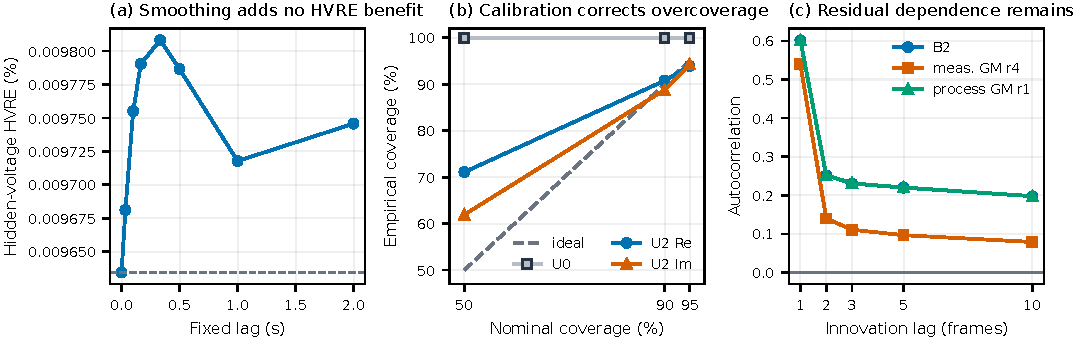
\includegraphics[width=\textwidth]{figures/generated/temporal_uncertainty.pdf}
\caption{Secondary temporal and uncertainty diagnostics for B2/B3 and calibration variants. These panels diagnose model adequacy; they do not upgrade nominal marginal coverage to a complete uncertainty claim.}
\label{fig:supp-temporal-uncertainty}
\end{figure*}

\begin{table}[t]
\caption{Median B2 hidden-bus TVE at the largest mismatch scale, $m=1.5$. Ratios use the 140-case main-grid nominal median of 0.014744\%.}
\label{tab:mismatch-results}
\centering
\footnotesize
\begin{tabular}{lcc}
\toprule
Mismatch family & TVE (\%) & Ratio \\
\midrule
M1 network & 0.250430 & 16.985$\times$ \\
M2 machine & 0.014744 & 1.000$\times$ \\
M3 governor & 0.014743 & 1.000$\times$ \\
M4 AVR & 0.014744 & 1.000$\times$ \\
M5 load model & 0.014761 & 1.001$\times$ \\
M6 operating point & 0.122641 & 8.318$\times$ \\
M7 coupled & 0.023615 & 1.602$\times$ \\
\bottomrule
\end{tabular}
\end{table}


\begin{table}[t]
\caption{Sign-pooled weak load-event TEST results for the frozen W2/L2 model. Each row contains 1,600 event cases (16 source buses, two signs, 50 noise replicas); the false-positive rate uses 800 no-event records.}
\label{tab:load-weak-results}
\centering
\scriptsize
\setlength{\tabcolsep}{3.2pt}
\begin{tabular}{cccccc}
\toprule
$|a|$ (\%) & AUROC & FPR (\%) & FNR (\%) & Top-1 (\%) & Top-3 (\%) \\
\midrule
0.010 & 0.733 & 0.25 & 83.1 & 13.0 & 37.1 \\
0.020 & 0.906 & 0.25 & 45.0 & 31.8 & 69.0 \\
0.050 & 0.995 & 0.25 & 4.5 & 73.4 & 95.9 \\
0.100 & 1.000 & 0.25 & 0.2 & 93.2 & 99.4 \\
0.200 & 1.000 & 0.25 & 0.0 & 98.9 & 100.0 \\
0.400 & 1.000 & 0.25 & 0.0 & 100.0 & 100.0 \\
\bottomrule
\end{tabular}
\end{table}


\begin{figure*}[t]
\centering
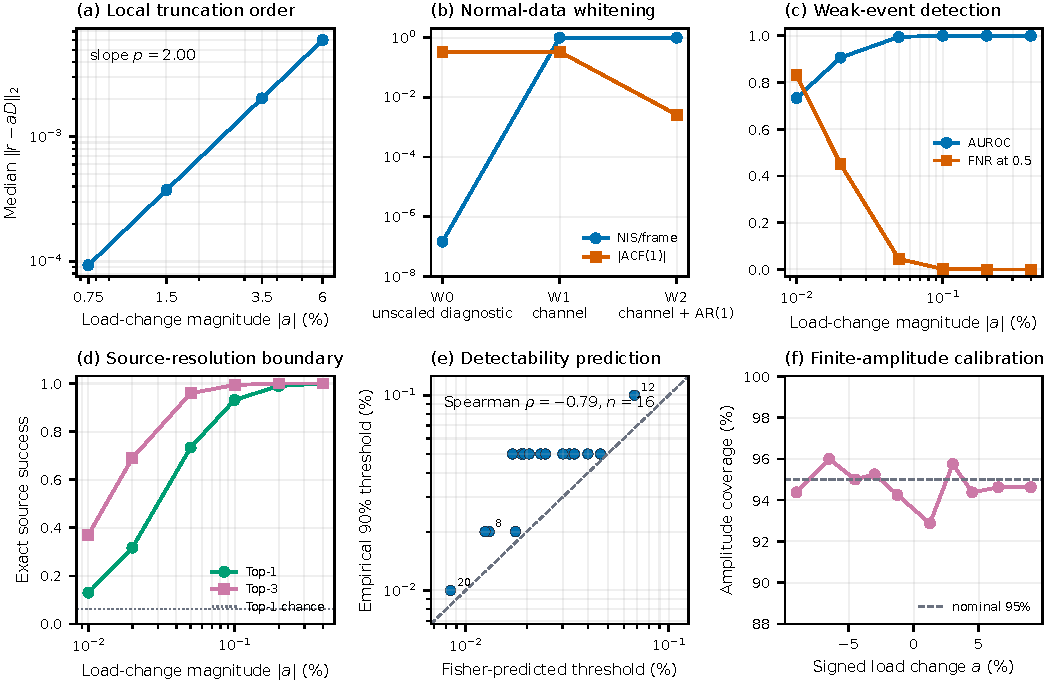
\includegraphics[width=\textwidth]{figures/generated/load_event_inference.pdf}
\caption{Single-source development evidence for the frozen load likelihood. The figure is retained as component validation; GLOBAL-137 in the main paper is the prospective support-recovery result.}
\label{fig:supp-load-inference}
\end{figure*}

\begin{table*}[t]
\caption{Audited sequential event-diagnosis baseline on the known-source TEST split, mean over three fitted seeds. The independent split unit is the complete trajectory; timestamp-level scores retain the denominators of the frozen evaluator.}
\label{tab:legacy-event-results}
\centering
\footnotesize
\begin{tabular}{lcccccc}
\toprule
Configuration & Detection F1 & Event macro-F1 & Physical Top-1 & Physical Top-3 & Integrity Top-1 & False alarms/min \\
\midrule
136-feature hierarchy & 0.965 & 0.791 & 0.496 & 0.646 & 0.870 & 4.01 \\
448-feature hierarchy & 0.975 & 0.815 & 0.590 & 0.717 & 0.865 & 1.45 \\
448 features + availability & 0.989 & 0.905 & 0.592 & 0.719 & 0.974 & 1.45 \\
\bottomrule
\end{tabular}
\end{table*}


\begin{figure*}[t]
\centering
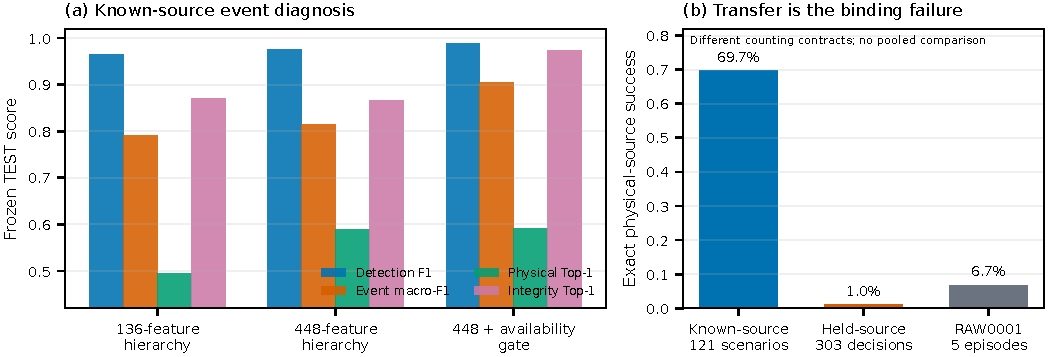
\includegraphics[width=\textwidth]{figures/generated/legacy_event_evidence.pdf}
\caption{Secondary evidence for the supervised ANDES baseline, including known-source performance and the source-holdout failure.}
\label{fig:supp-legacy}
\end{figure*}

\clearpage
\bibliographystyle{IEEEtran}
\bibliography{references}
\EOD
\end{document}
